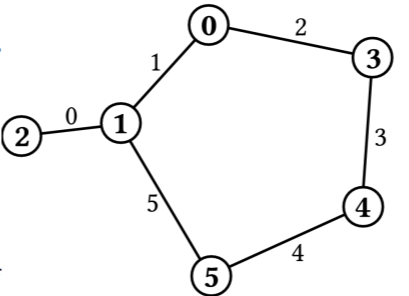
\includegraphics{garden1.png}

There are only two possible valid routes in the first example that follow 3 trails:
$1 \rightarrow 2 \rightarrow 1 \rightarrow 0$, and $5 \rightarrow 4 \rightarrow 3 \rightarrow 0$. The first route starts at fountain 1. The most beautiful trail from here leads to fountain $2$. At fountain $2$, the group has no choice, they must return using the same trail. Back at fountain 1, the group will now avoid trail 0 and choose trail 1 instead. This trail does indeed bring them to the fountain $P=0$. Thus, the procedure should call \t{answer(2)}.

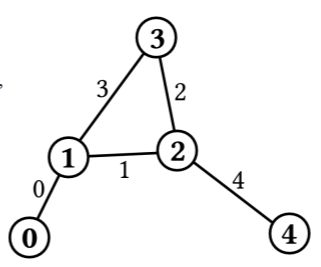
\includegraphics{garden2.png}


For the first group in the second example, there is only one valid route that reaches
fountain $2$ after following 3 trails: $1 \rightarrow 0 \rightarrow 1 \rightarrow 2$.
For the second group, there are two valid routes that reach fountain 2 after following $1$ trail: $3 \rightarrow 2$, and $4 \rightarrow 2$. Therefore, the correct implementation of \t{count\_routes} should first call \t{answer(1)} to report the answer for the first group, and then call \t{answer(2)} to report the answer for the second group.